\documentclass[10pt]{report}
\usepackage{fancyhdr}
\usepackage{amsmath}
\usepackage{graphicx}
\graphicspath{ {./} }

\pagestyle {fancy}
\fancyhf{}
\rhead{Engineering Problem 6 - Investment | James Xu | 1006058855}
\rfoot{Page \thepage}

\begin{document}
    \section*{The Plan}
    \subsection*{Problem Statement}
    A program is required to interpret investment and compound interest (compounded discretely and continuously) mathematically, to compute the future value of an investment given some parameters for contract term and interest rate, as well as graphically displaying the value against time for a given set of parameters.

    \subsection*{Goals}
    \begin{enumerate}
        \item Computation of the payoff with both discretely and continously compounding interest of an initial payment of \$100, a rate of 0.05 and a time period of 5.5 years using Matlab
        \item Set the program to compute the values given variable rate and time values.
        \item Plot of final value against time for specific values (principle = \$1, t: 1 to 35 years, r = 0.08, $t_{stepsize} = $0.5 year)
    \end{enumerate}
    \subsection*{Foundations}
    The equation to compute these discrete compounded value is $$\text{final value} = \text{principal} \times (1+ \frac{r}{m})^{mt}.$$ Interestingly, the discrete value, given as $\lim_{m\to\infty}$ resembles euler's number, and indeed returns a function of $e$ (which makes sense as this will be an exponentially growing function). For reference, $$e = \lim_{m \to\infty}(1 + \frac{1}{m})^m$$ The continuous compounded value is given by $$\text{final value} = \text{principal} \times e^{rt}$$ Some reasonable ranges for interest rates would be from maybe around -5\% (though negative interest is rare) to 20\%, which will reasonably capture most benchmark interest rates in recent history in most countries. (This is the interest rate from the central bank lending to commercial banks). A reasonable range for time is 1 to 60 years, just as a guess of how long people might save for.\\\\

    \section*{Process}
    First, all the variables are declared:
    \begin{itemize}
        \item vi = principle, intial monetary input
        \item r = interest rate
        \item t = time period over which interest accumulates
        \item m = number of periods per year (kept constant; m = 2)
        \item vo = final value of investement after t years and r interest rate
    \end{itemize}

    For goal (1) - the values can be computed directly by inputting the given principal, r, and t, setting m as 2. The computation can be carried out in simply matlab by assigning the appropriate values for the variables and plugging them into the two equations given.\\\\
    For goal (2) - The variables for r and t are initialized as vectors and assigned via the \textit{linspace} keyword a range of values that are reasonable. Using a nested for loop and string formatting (\textit{sprintf}), a list of ouptuts is generated comparing each interest rate and time period, and outputted to the console. They are evaluated with both the continuous and discrete methods.\\\\
    For goal (3), some thinking is required to create a stairstep graph for the discretely evaluated compound interest. While Matlab might have some ways to do this internally, I came up with a somewhat elegant way to compute this. This subproblem was one of rounding the time value to the closest half year, so I designed this equation: $$round_{\frac{1}{2}}(x) = \frac{\left \lfloor{2x}\right \rfloor }{2}$$ utilizing the properties of the floor (round down) function to round down the value to the closest half. \\ Graphing the value of the continuously evaluated function was trivial, just plotting t against f(t), where f(t) is given in the Foundations for continous compounded value. Plotting the discretely evaluated function required me to alter the t value, smoothing it to a stairstep using the $round_{\frac{1}{2}} (t)$ and evaluate $f_d(t)$ again using the appropriate equation given in the Foundations section.


    \section*{Conclusion}
    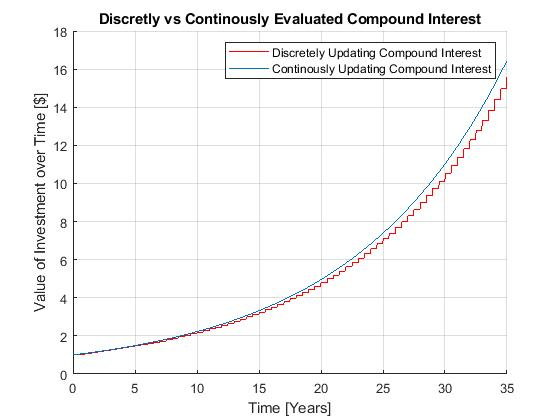
\includegraphics[width=\textwidth]{graph_final_2d.jpg}

    \section*{$\frac{1}{2}$ Page Critique of Computer Aided Problem Solving}

    - Computers can take some input and generate an output
    - With properly defined input and instructions, a computer can expedite the problem solving process, as sometimes problem solving requires one to obtain numeric values or visualizations that are otherwise extremely tedious

\end{document}
